\subsection{Spymaster's Turn Scenario}
A major part of the Codenames game is the Spymasters giving clues. In our design the simulated players are objects, and the GameManager calls their makeMove() functions to trigger them to play the game. In the case of the Spymaster, the GameManager tells the Spymaster to make a move, expecting it to return a clue. Following the Strategy design pattern, a Spymaster may implement different strategies for generating this clue. The Spymaster calls on its specific SpyStrategy object to create the clue returning the clue to the GameManager.


\begin{figure}[H]
\centering
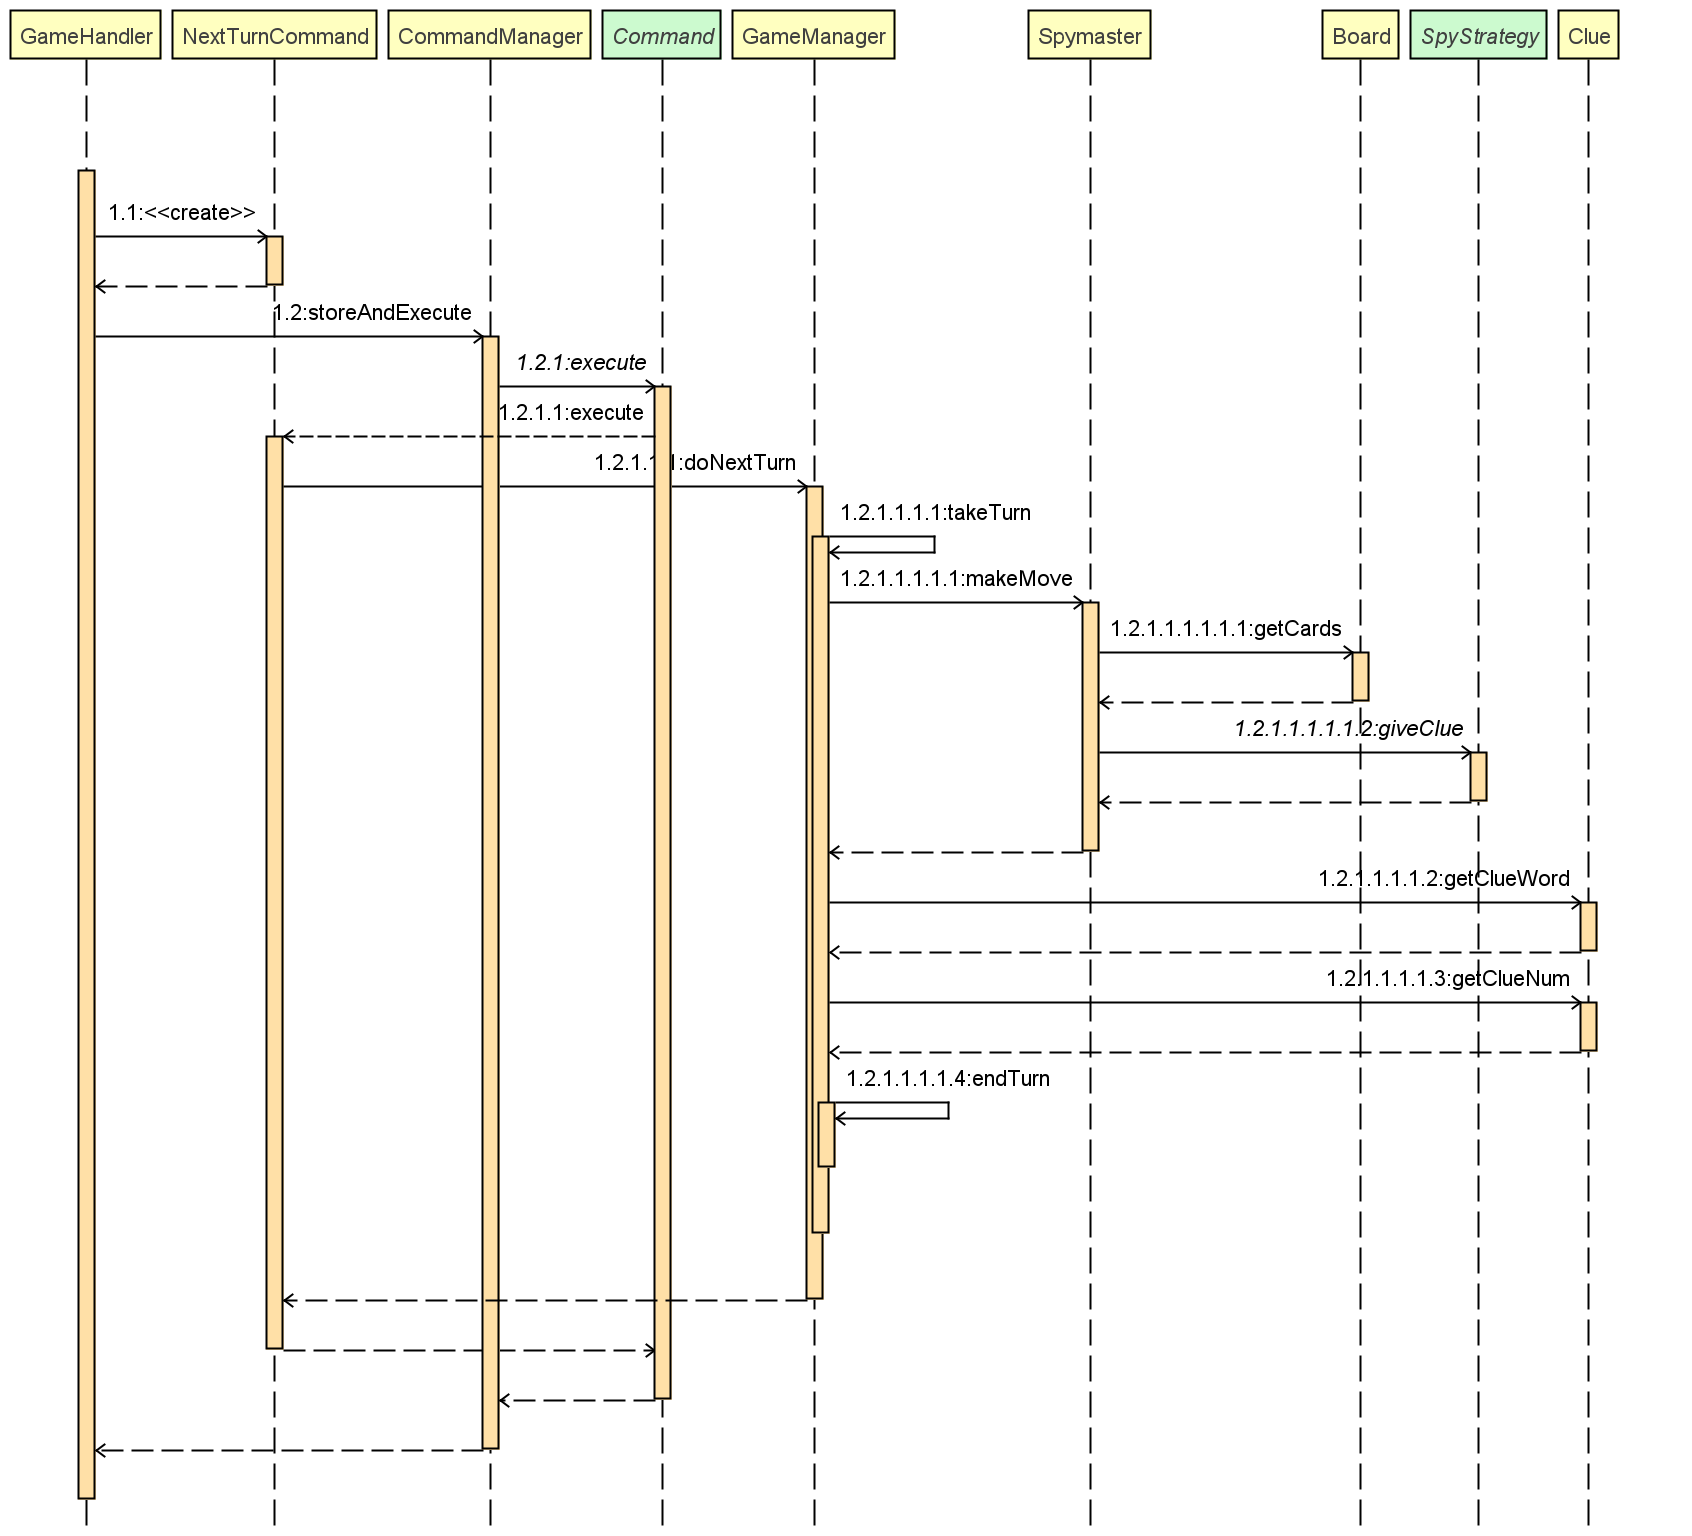
\includegraphics[width=10cm]{Source/DynamicDesign/Scenario/Spymaster.png}
\caption{Sequence Diagram of Spymaster}
\end{figure}